\section{Physikalische Grundlagen}
Die Ausführungen in diesem Abschnitt orientieren sich an \cite{manual}.
%TODO add manual to bibtex

\subsection{Semiklassische Erklärung des Hanle-Effekts}

Semiklassisch wird der Hanle-Effekt folgendermaßen erklärt:
Wenn linear polarisiertes Licht (konstante Richtung von $\vec{\text{E}}$- und $\vec{\text{B}}$-Feld)
ein Atom anregt, ist für dieses angeregte Atom die Richtung seines Dipolmoments $\vec{P}$ vorgegeben:
Es zeigt in Richtung des $\vec{\text{E}}$-Feldes. Senkrecht dazu steht das magnetische Moment $\vec{\mu}$.
\autoref{img:rotation} zeigt den Zusammenhang.\\

\begin{figure}[H]
\begin{center}
  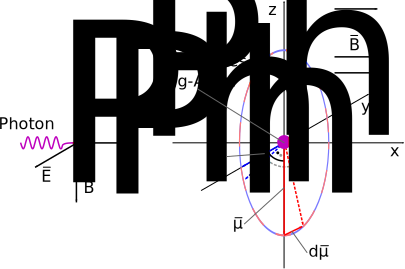
\includegraphics[width=0.5\textwidth]{../img/rotation.pdf}
  \caption{Hanle-Effekt: Präzession des magnetische Moments $\vec{\mu}$ eines angeregten Atoms im
  Magnetfeld $\vec{B}$. Das Dipolmoment $\vec{P}$ steht senkrecht auf $\vec{\mu}$ und rotiert mit.}
  \label{img:rotation}
\end{center}
\end{figure}

Wenn kein äußeres Magnetfeld vorhanden ist,
hat das angeregte Atom die gewöhnliche Abstrahlcharakteristik eines Hertzschen Dipols:
Die Intensität der abgestrahlten Leistung $I$ zeigt eine sin$^2$-Abhängigkeit vom Winkel $\varphi$ zur
Dipolachse:
\begin{equation}
\label{eq:hertz}
I(\varphi) \propto \sin^2(\varphi)
\end{equation} 
\autoref{img:dipol} zeigt diese Abstrahlcharakteristik.

\begin{figure}[H]
\begin{center}
  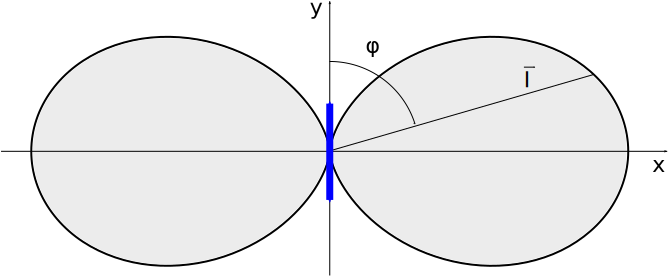
\includegraphics[width=0.6\textwidth]{../img/dipol.pdf}
  \caption{Abstrahlcharakteristik eines Hertzschen Dipols: Strahlungsintensität $\vec{I}$ in Abhängigkeit des
  Winkels $\varphi$.}
  \label{img:dipol}
\end{center}
\end{figure}

Ein einzelnes angeregtes Atom fällt mit der Wahrscheinlichkeit $\exp(-\frac{\tau}{t})$ zurück in den Grundzustand.
(Die mittlere Lebensdauer des angeregten Atoms wird mit $\tau$ bezeichnet, die Anregung findet bei $t = 0$ statt.)
Damit erhält man für die winkelabhängige Gesamtintensität
\begin{equation}
\label{eq:int}
I(\varphi) = A \cdot \int_0^{\infty} \sin^2(\varphi) \cdot \text{e}^{-\frac{\tau}{t}} \ \text{d}t \, \ .
\end{equation}
$A$ ist hier eine Konstante. Befindet sich das angeregte Atom allerdings in einem Magnetfeld $\vec{\text{B}}$,
ist das Integral nicht mehr einfach zu lösen, weil der Winkel $\varphi$ dann zeitabhängig ist.
Dies wird verursacht durch das Drehmoment, das von dem Magnetfeld auf das System ausgeübt wird.
Es gilt
\begin{equation}
\label{eq:dmu}
\frac{\text{d}\vec{\mu}}{\text{d}t} = \frac{\omega_L}{B} \cdot (\vec{\mu} \times \vec{\text{B}}) \ \, .
\end{equation}
Die Änderung von $\vec{\mu}$  führt zu einer Präzession in der Ebene senkrecht zum Magnetfeld
mit der Larmorfrequenz $\omega_L$.
Sie ist abhängig von der Stärke des Magnetfelds, es gilt
\begin{equation}
\label{eq:larmorfreq}
\omega_L = B \cdot \frac{g_J \cdot \mu_B}{\hbar} \ \, .
\end{equation}
Da das Dipolmoment $\vec{P}$ fest mit $\vec{\mu}$ verbunden ist, präzediert auch dieses, und es gilt für den
Winkel
\begin{equation}
\label{eq:phit}
\varphi(t) = \omega_L \cdot t \ \, .
\end{equation}
Die Winkel- und Magnetfeldabhängigkeit der Intensität wird also von folgendem Integral beschrieben:
\begin{equation}
\label{eq:int}
I(\Phi,B) = A \cdot \int_0^{\infty} \sin^2 \left( \frac{g_J \cdot \mu_B}{\hbar} \cdot (B-B_0) \cdot t + \Phi \right) \cdot
\text{e}^{-\frac{\tau}{t}} \ \text{d}t + c \, \ .
\end{equation}
$\Phi$ ist der Winkel zwischen der Polarisationsachse des eingestrahlten Lichts und der Richtung,
in der sich der Strahlungsdetektor befindet.
$A$, $B_0$ und $c$ sind hier Konstanten, die die Amplitude und Offsets der Messdaten beschreiben.
Die Lösung des Integrals lautet
\begin{equation}
\label{eq:intensity}
I(\Phi,B) = A \tau \cdot \frac{2 a \tau  (B-B_0) \sin (2 \Phi )+(2 a \tau  (B-B_0))^2-\cos (2 \Phi )+1}
{2 \left((2 a \tau  (B-B_0))^2+1\right)}+c \ ,
\end{equation}
mit
\begin{equation}
\label{}
a=\frac{g_J \cdot \mu_B}{\hbar} \, \ .
\end{equation}

\subsection{Quantenmechanische Erklärung des Hanle-Effekts}

\subsection{\emph{Coherence Narrowing} und Dampfdruck}